\documentclass{article}
\usepackage{xcolor}
\usepackage{tikz}
\usepackage{graphicx}


\begin{document}
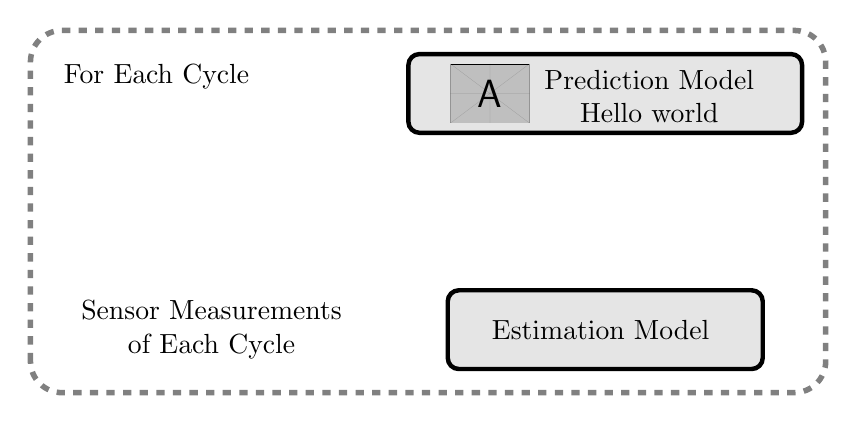
\begin{tikzpicture}
  \draw[draw=none] (-2.0, -0.5) rectangle (2.0, 0.5);
  \node[align=center] at (0.0, 0.0) { Sensor Measurements\\of Each Cycle };
  \draw[fill=black!10, rounded corners=4pt, ultra thick] (3.0, -0.5) rectangle (7.0, 0.5);
  \node[align=center] at (5.0, 0.0) { Estimation Model };
  \draw[fill=black!10, rounded corners=4pt, ultra thick] (2.5, 2.5) rectangle (7.5, 3.5);
  \node at (5.0, 3.0) {
    \hbox{
      \raisebox{.0\height}{\includegraphics[width=1cm]{example-image-a}} 
      \vbox{\hbox to 8em{\hfill Prediction Model\hfill}\hbox to 8em{\hfill Hello world\hfill}}
    }
  };
  % \node[align=center, anchor=west] at (5.0, 3.0) { Prediction Model };
  \draw[draw=gray, dashed, line width=2pt, rounded corners=4mm] (-2.3, -0.7999999999999998) rectangle (7.8, 3.8);
  \node[anchor=north west, align=center] at (-1.9999999999999998, 3.5) { For Each Cycle };
\end{tikzpicture}
\end{document}